\documentclass[30pt]{beamer}
\usepackage{graphicx, epstopdf}
\graphicspath{{Fig/}}
\usepackage{adjustbox}
\usepackage{tikz, flowchart}
\usetikzlibrary{shapes, patterns}
\usepackage{xcolor}
\definecolor{myblue}{rgb}{0.137,0.466,0.741}

\usetheme{Amsterdam}
\author{ Hsuan-Wei Lee,
  Anzhelika Lyubenko,
  Yuhang Ma,
  Emily Meissen,
  Daniela Velez-Rendon,
    Nara Yoon \newline \newline \underline{Mentors:} \newline John Peach, \newline Cammey Cole Manning,\newline Christian Gunning}


%\vspace{.1truein}

\title[]{Modeling Ebola: System, Agent, and Spatial Models}


%\date{February 28, 2015}

\begin{document}

\begin{frame}[t,plain]
    \titlepage
    \begin{center}
Mentors:\\John Peach\\ Cammey Cole Manning\\
Christian Gunning
\end{center}
\end{frame}

\begin{frame}[t,plain]
    \frametitle{Overview}
    \setbeamerfont*{itemize/enumerate body}{size=\Large}
\setbeamerfont*{itemize/enumerate subbody}{parent=itemize/enumerate body}
\setbeamerfont*{itemize/enumerate subsubbody}{parent=itemize/enumerate body}
\begin{enumerate}
\vfill
\item Introduction\vspace{2mm}
\item Models
\begin{itemize}
\item System-based
\item Agent-based
\item Spatial agent-based
\end{itemize}
\item Comparison
\item Summary
\end{enumerate}
\end{frame}

\begin{frame}
\frametitle{Introduction}
\section{Intro}
\begin{itemize}
\item Ebola was discovered in 1976
\item Early symptoms:  headache, fatigue, joint pain
\item Later symptoms: abdominal pain, diarrhea, vomiting, rashes
\item Diseases like HIV and Malaria have the same symptoms
\item The virus is contracted through direct contact with bodily fluids and secretion
\item Incubation period may last up to two weeks
\item Serious outbreaks in Liberia, Sierra Leone, and Guinea (2014)
\end{itemize}
\end{frame}



\begin{frame}
\frametitle{Compartment Model of the Ebola Epidemic in Liberia}
\section{Models}

\begin{figure}[!h]
  \centering
  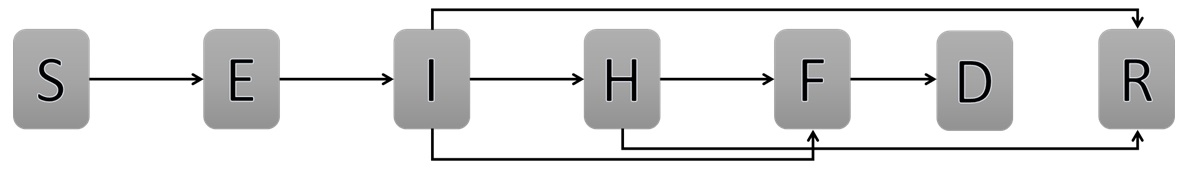
\includegraphics[width=1\textwidth]{compartmentNoFlow}
 \label{fig:compartment} 
\end{figure}

\begin{center}
\begin{tabular}{l l}
 S:& Susceptible\\
 E:& Exposed \\
 I:& Infectious \\
 H:& Hospitalized \\
 F:& Funeral  \\
 R:& Recovered \\
 D:& Dead 
\end{tabular}
\end{center}
\end{frame}



\begin{frame}
\frametitle{Assumptions}
\begin{itemize}
\item Focus on Liberia in 2014-2015
\item Closed system
\item Everyone who dies has a traditional funeral
\end{itemize}
\end{frame}



\begin{frame}
\frametitle{System Dynamics Differential Equations}
\section{System}
\begin{align*} 
\label{SDeqn}
\frac{dS}{dt} &= - \frac{\beta_{I}SI+\beta_{H}SH+\beta_{F}SF}{N} \\
\frac{dE}{dt} &=  \frac{\beta_{I}SI+\beta_{H}SH+\beta_{F}SF}{N}-\gamma_P E \\
\frac{dI}{dt} &=  \gamma_P E - [\gamma_{H}\theta + \gamma_{I}(1-\theta)(1-\delta_{1})+\gamma_{D}(1-\theta)\delta_{1}]I \\
\frac{dH}{dt} &= \gamma_{H}\theta I - [\gamma_{HF}\delta_{2}+\gamma_{IH}(1-\delta_{2})]H\\
\frac{dF}{dt} &= \gamma_{D}(1-\theta) \delta_{1} I + \gamma_{DH}\delta_{2} H-\gamma_{F} F \\
\frac{dR}{dt} &= \gamma_{I}(1-\theta)(1- \delta_{1}) I + \gamma_{HR}(1-\delta_{2}) H\\
\frac{dD}{dt} &= \gamma_{F} F 
\end{align*}
\end{frame}



\begin{frame}
\frametitle{Model Parameters for Ebola Epidemic in Liberia}
\begin{table}[ht]
\centering % used for centering table
\resizebox{.8\linewidth}{!}{
\begin{tabular}{c c}
\hline\hline %inserts double horizontal lines
Parameter & Value\\ [0.5ex]
\hline % inserts single horizontal line
Incubation Period (${t_{P}}$) & 11 days\\
Duration of Traditional Funeral (${t_{F}}$) & 2.00 days\\
Time from Infection to Recovery (${t_{I}}$) & 10.00 days\\
Time from Infection to Death (${t_{D}}$) & 8.00 days\\
Case Fatality Rate, Unhospitalized ($\delta_{1}$) & 0.500\\
Case Fatality Rate, Hospitalized ($\delta_{2}$) & 0.500\\\hline
\end{tabular}}
\end{table}

\begin{table}[ht]
\centering % used for centering table
\resizebox{\linewidth}{!}{
\begin{tabular}{c c c}
\hline\hline %inserts double horizontal lines
Parameter &  Before Intervention  & After Intervention \\ [0.5ex]
 & (Mar 2014 to Sept 2014) &  (Sept 2014 to July 2015) \\ [0.5ex] % inserts table
% inserts table
%heading
\hline % inserts single horizontal line
{Contact Rate, Community  (${\beta_{I}}$) }& {0.148 (0.0953)} & {0.0446 (0.0338)}\\
Contact Rate, Hospital  ($\beta_{H}$) & 0.235 (0.143) & 0.0877 (0.0563) \\
Contact Rate, Funeral  ($\beta_{F}$) & 0.465 (0.287)& 0.283 (0.208)  \\
Time until Hospitalization (${t_{H}}$) & 4.49 (1.44) days & 4.63 (1.43) days  \\
Time from Hospitalization to Death (${t_{DH}}$) & 3.51 (1.44) days & 3.51 (1.43) days  \\
Time from Hospitalization to Recovery (${t_{IH}}$) & 5.51 (1.44) days & 5.51 (1.43) days  \\
Probability a Case is Hospitalized ($\theta$) & 0.248 (0.142) & 0.233 (0.145) \\
[1ex]
\hline
\end{tabular}}
\end{table}
\end{frame}



\begin{frame}
\frametitle{World Health Organization Data vs. Systems Model}
\begin{figure}[!h]
  \centering
  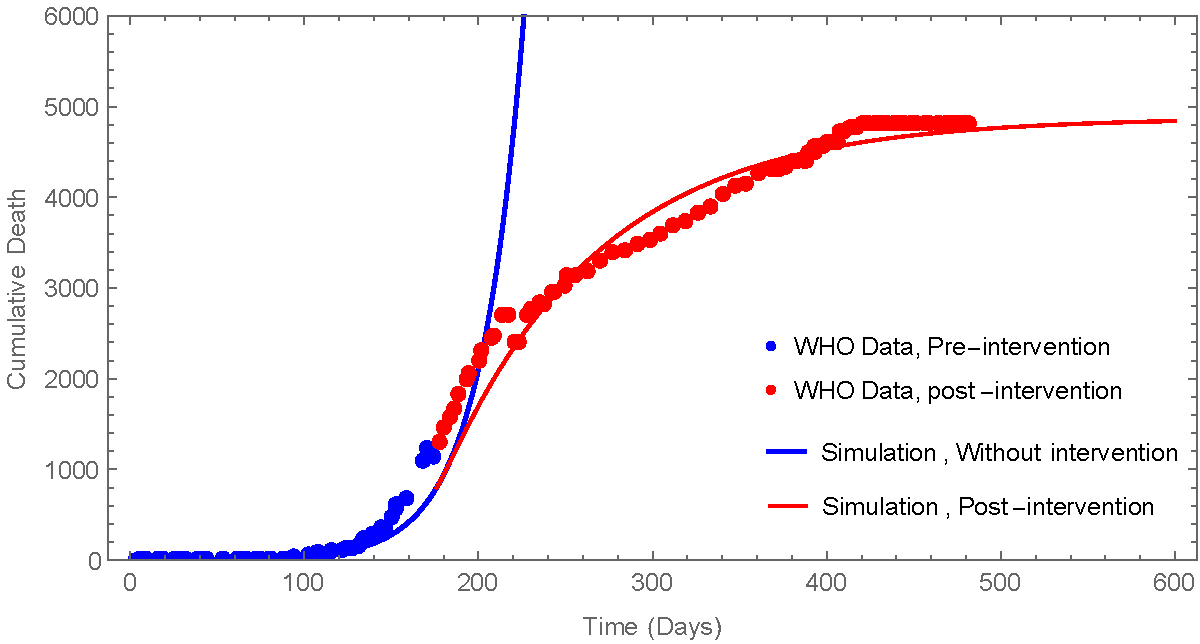
\includegraphics[width=1\textwidth]{ValidationPlot.pdf}
 \end{figure}
\end{frame}



\begin{frame}
\frametitle{System Model Results: With and Without Intervention}
\begin{figure}[!h]
  \centering
  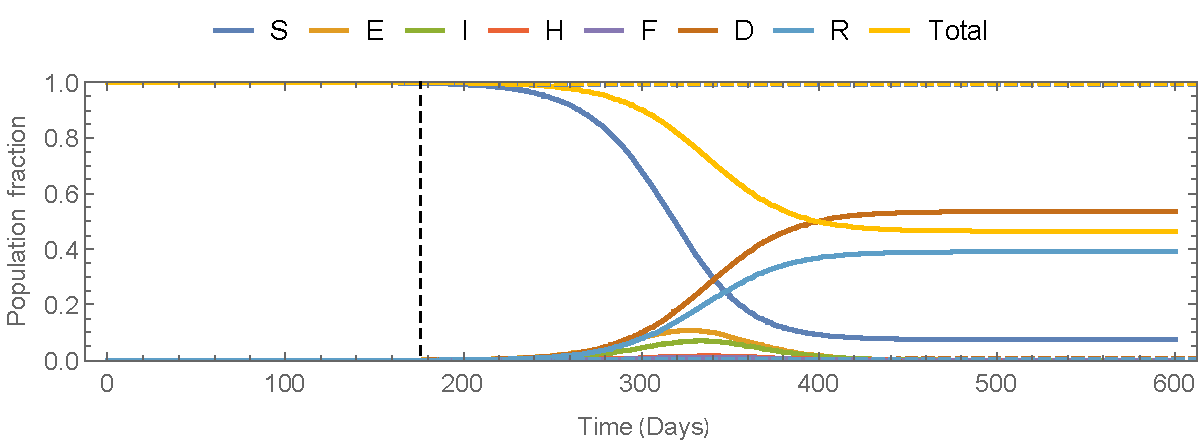
\includegraphics[width=1\textwidth]{SEIPlot.pdf}
\label{fig:LB_IM_NoIn} 
 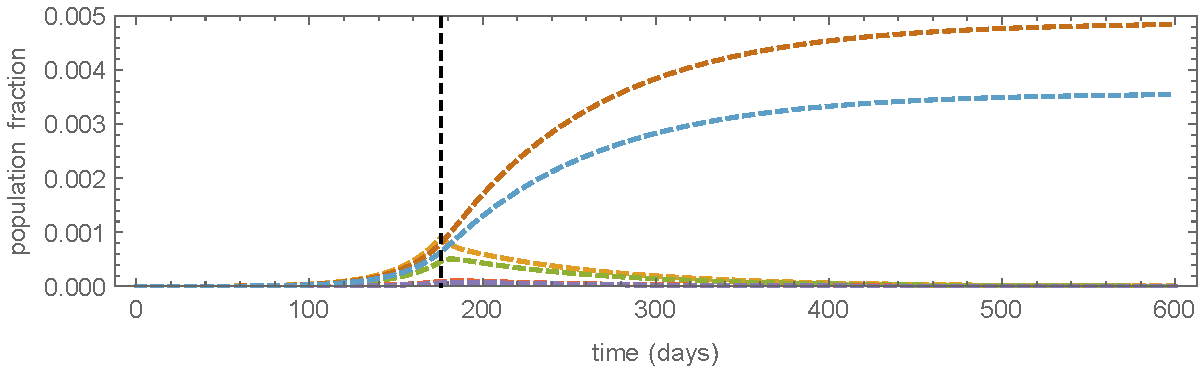
\includegraphics[width=\textwidth]{SEIPlotIntRescale.pdf}  \label{fig:LB_IM_In2} %\end{subfigure} 
\label{fig:LB_IM_In} 
%\begin{frame}
%\frametitle{System Model Results}
%\begin{figure}[h!]
% \centering 
% \begin{subfigure}{\textwidth}
%  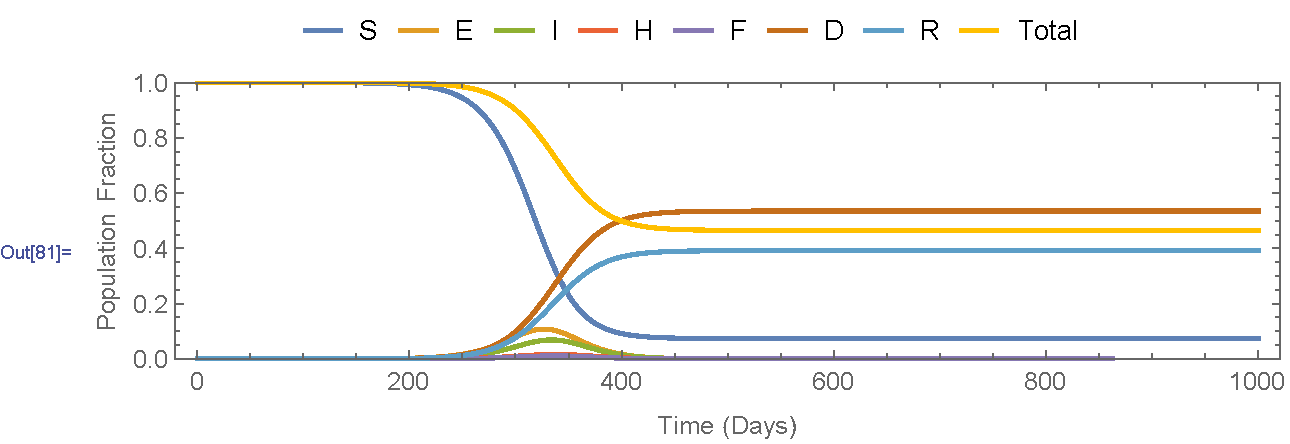
\includegraphics[width=\textwidth]{SEIPlotNoInt.pdf} 
%\end{subfigure}
%  \hspace{.1cm}
%\begin{subfigure}{\textwidth}
% 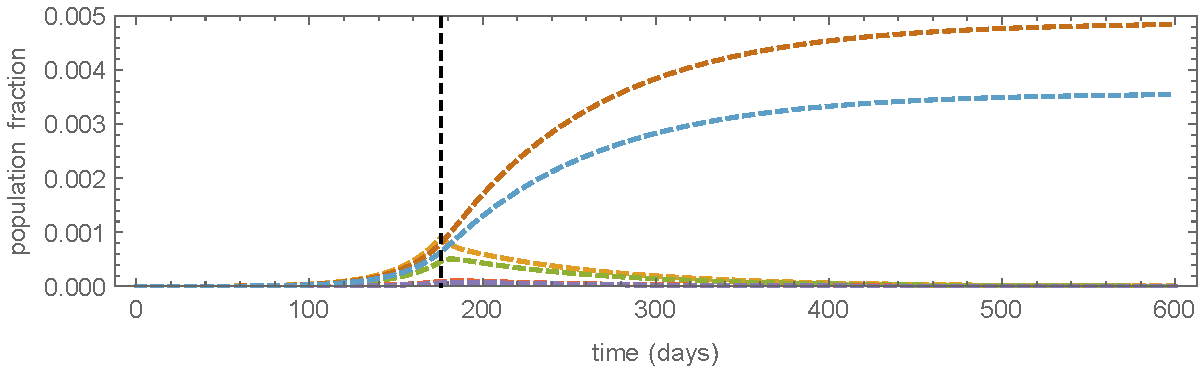
\includegraphics[width=\textwidth]{SEIPlotIntRescale.pdf}  
%\end{subfigure} 
\end{figure}
\end{frame}


%\begin{frame}
%\frametitle{System Model Results Post-treatment}
%\begin{figure}[h!]
% \centering 
%% \begin{subfigure}{\textwidth}
%  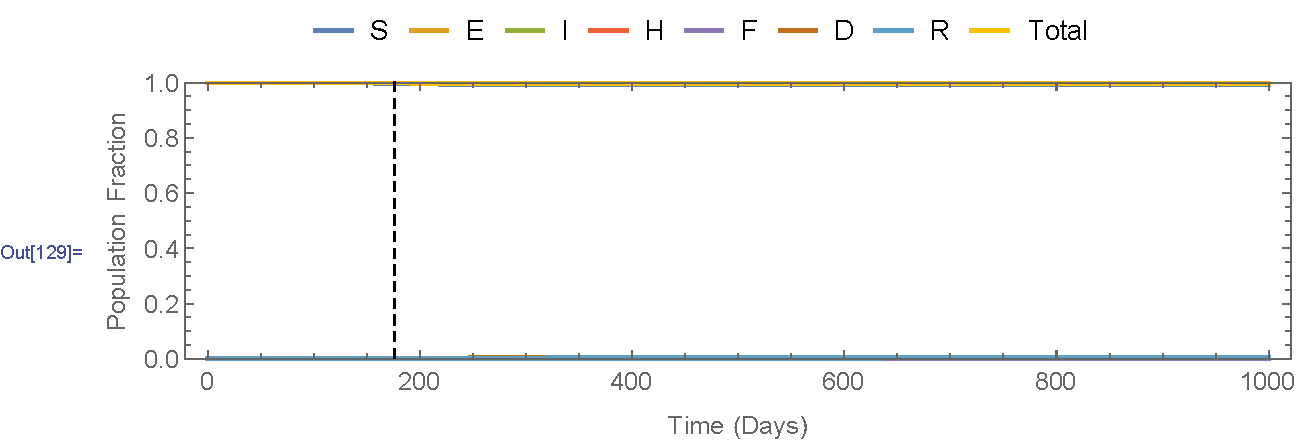
\includegraphics[width=\textwidth]{SEIPlotInt.pdf}  \label{fig:LB_IM_In1} %\end{subfigure}
%  \hspace{.1cm}
%%\begin{subfigure}{\textwidth}
%
%\end{figure}
%\end{frame}



\begin{frame}
\frametitle{Agent-based model}
\section{Agent}
%MAYBE INCLUDE DIAGRAM
%\begin{figure}
%\begin{tikzpicture}[->,>=stealth',shorten >=1pt,auto,node distance=3cm,
%  thick,main node/.style={circle,fill=blue!20,draw,font=\sffamily\Large\bfseries}]
%  \node[main node] (1) {S};
%  \node[main node] (2) [right of=1] {E};
%  \node[main node] (3) [right of=2] {I};
%  \node[main node] (4) [right of=3] {R};
%    \node[main node] (5) [below left of=3] {D};
%      \node[main node] (6) [below right of=3] {F};
%        \node[main node] (7) [right of=6] {H};
%
%  \path[every node/.style={font=\sffamily\small}]
%    (1)
%        edge node {$p_{SE}$} (2)
%        edge [loop above] node {$p_{SS}$} (1)
%    (2) 
%        edge node {$p_{EI}$} (3)
%         edge [loop above] node {$p_{EE}$} (2)
%      
%    (3) 
%       edge node {$p_{IR}$} (4)
%       edge node[left] {$p_{IF}$} (6)
%       edge node {$p_{IH}$} (7)
%        edge [loop above] node {$p_{II}$} (3)
%    (4)
%         edge [loop above] node {$p_{RR}$} (4)
%       
%(6) edge node{$p_{FD}$} (5) 
%edge [loop below] node {$p_{FF}$} (6)     
%(7) edge node[right]{$p_{HR}$} (4) 
%edge [loop below] node {$p_{HH}$} (7)
%  (7) edge node{$p_{HF}$} (6)      
% (5) edge [loop below] node {$p_{DD}$} (5)
%        ;
%\end{tikzpicture}
%\end{figure}
\begin{itemize}
%\item \textbf{INCLUDE FLOW CHART ONE MORE TIME}
\item System $\implies$ agent
\item Compartment $\implies$ state
\item Deterministic $\implies$ probabilistic
\item Simulation:
\begin{itemize}
\item 1000 individuals; 1 exposed
\item 300 days
\item 100 repetitions
\end{itemize}
\end{itemize}
\end{frame}


\begin{frame}
\frametitle{Probability of having an outbreak}
\vspace{5mm}
\textcolor{myblue}{outbreak}: 2\% of population contracts disease
\begin{figure}
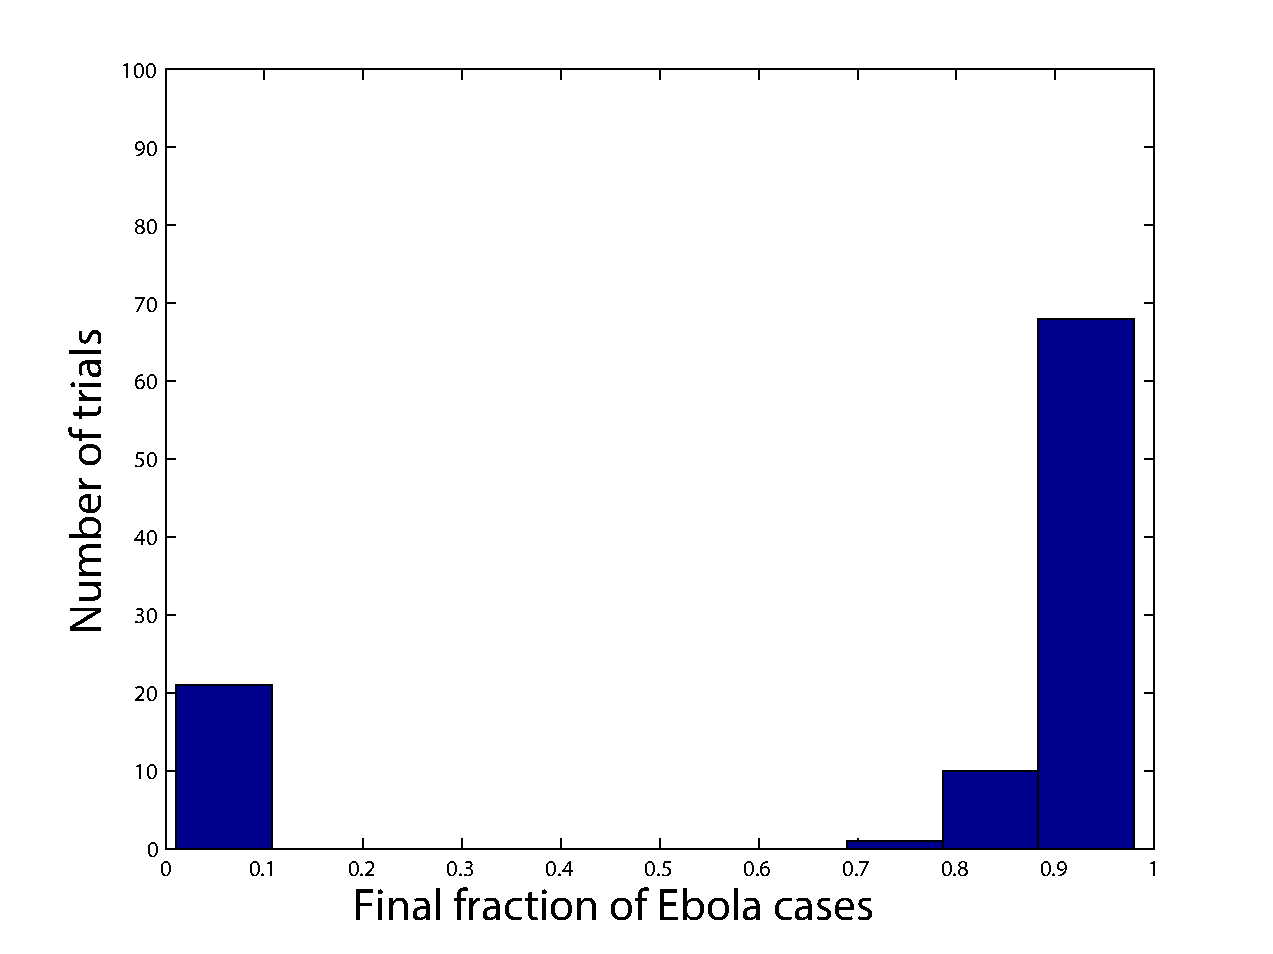
\includegraphics[width = 0.5\textwidth]{N100Hist.pdf}
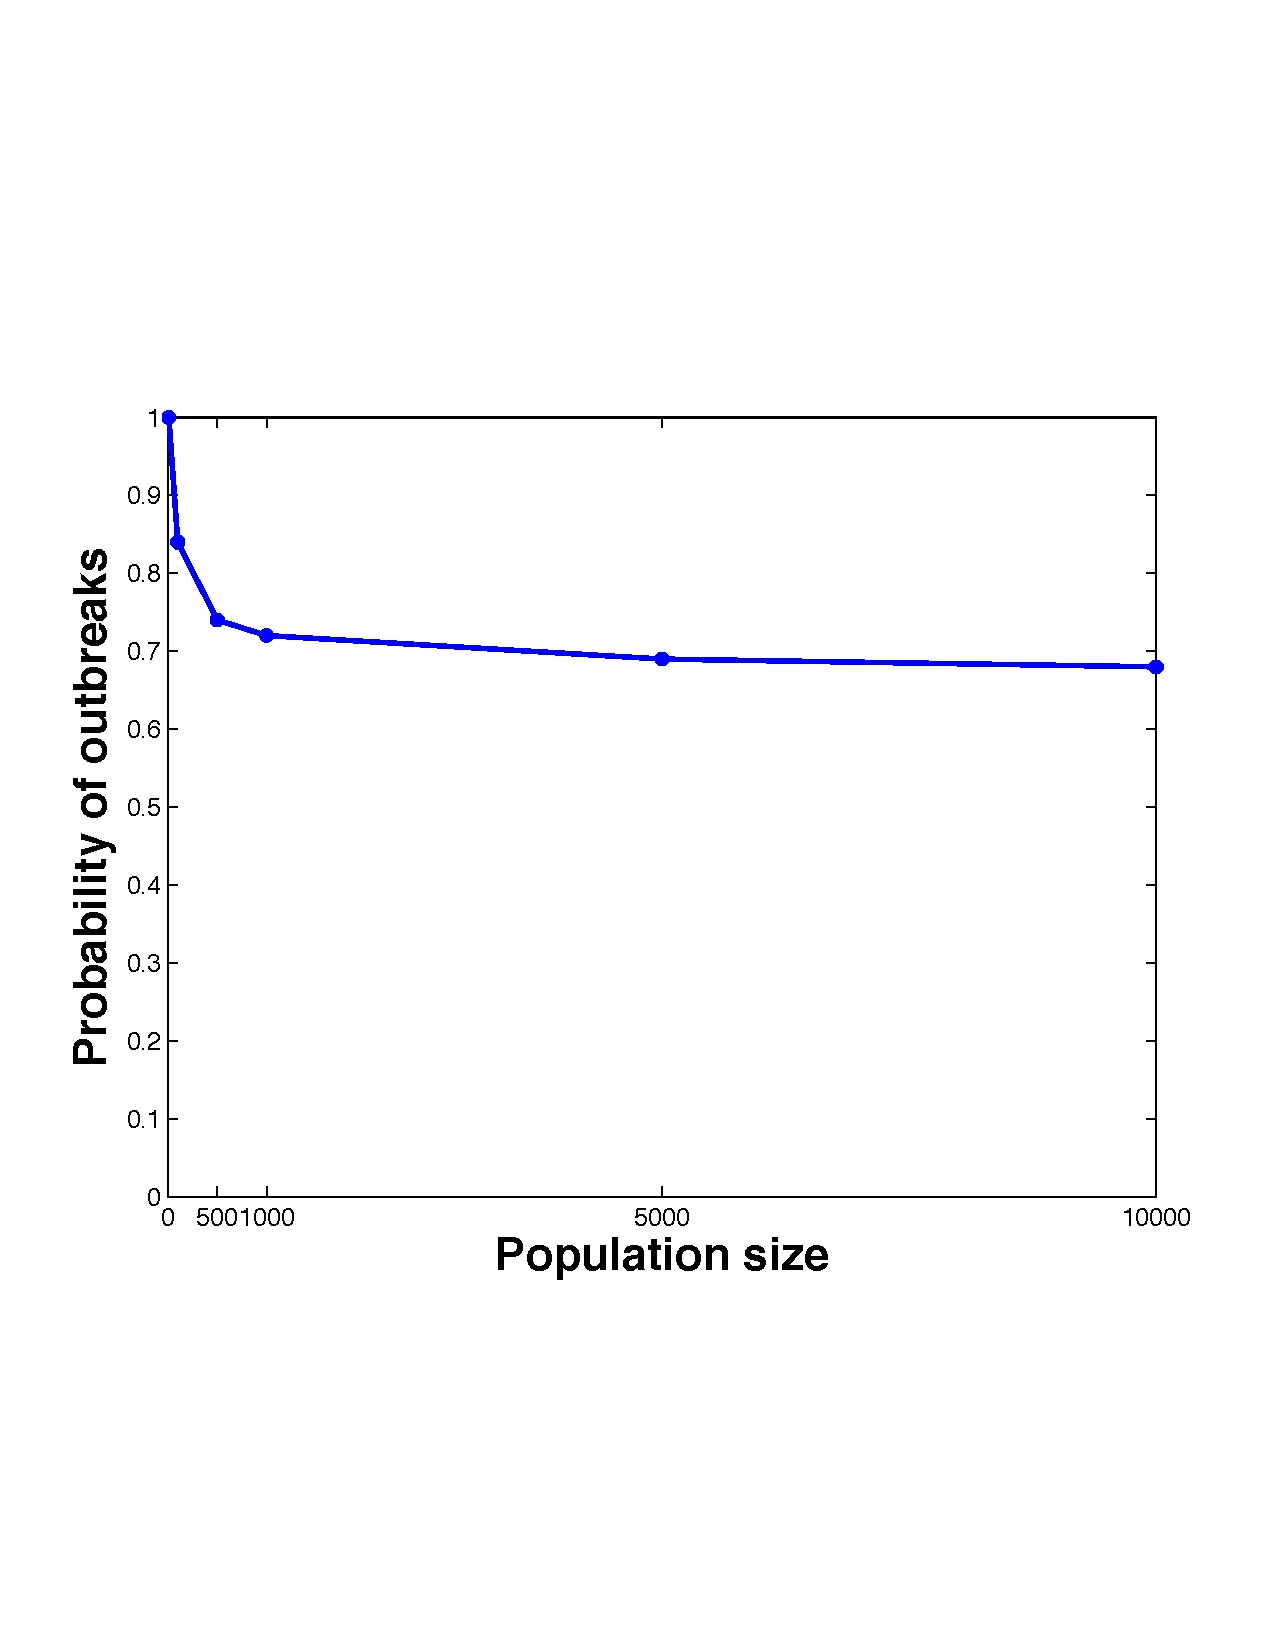
\includegraphics[width = 0.5\textwidth]{OutbreakProb.pdf}
\end{figure}
\end{frame}

\begin{frame}
\frametitle{Effects of Ebola outbreak}
\begin{figure}
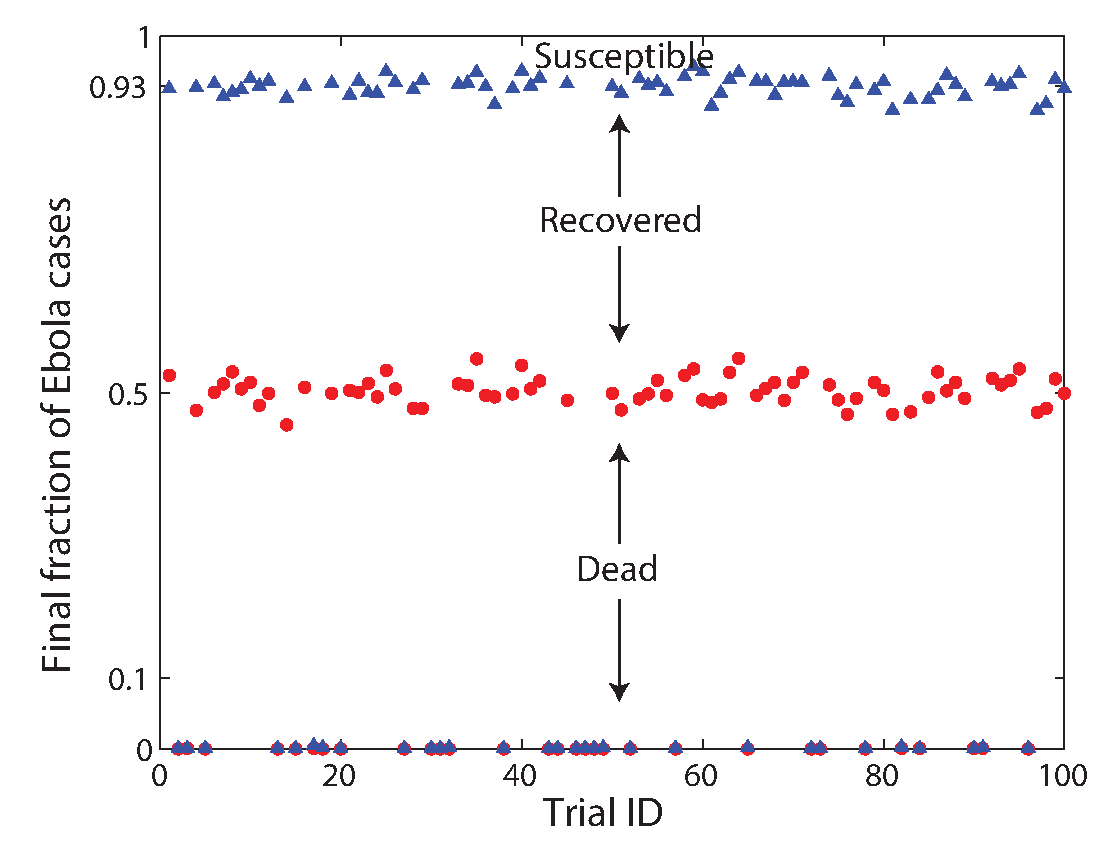
\includegraphics[width = 0.5\textwidth]{N1000Scatter.pdf}
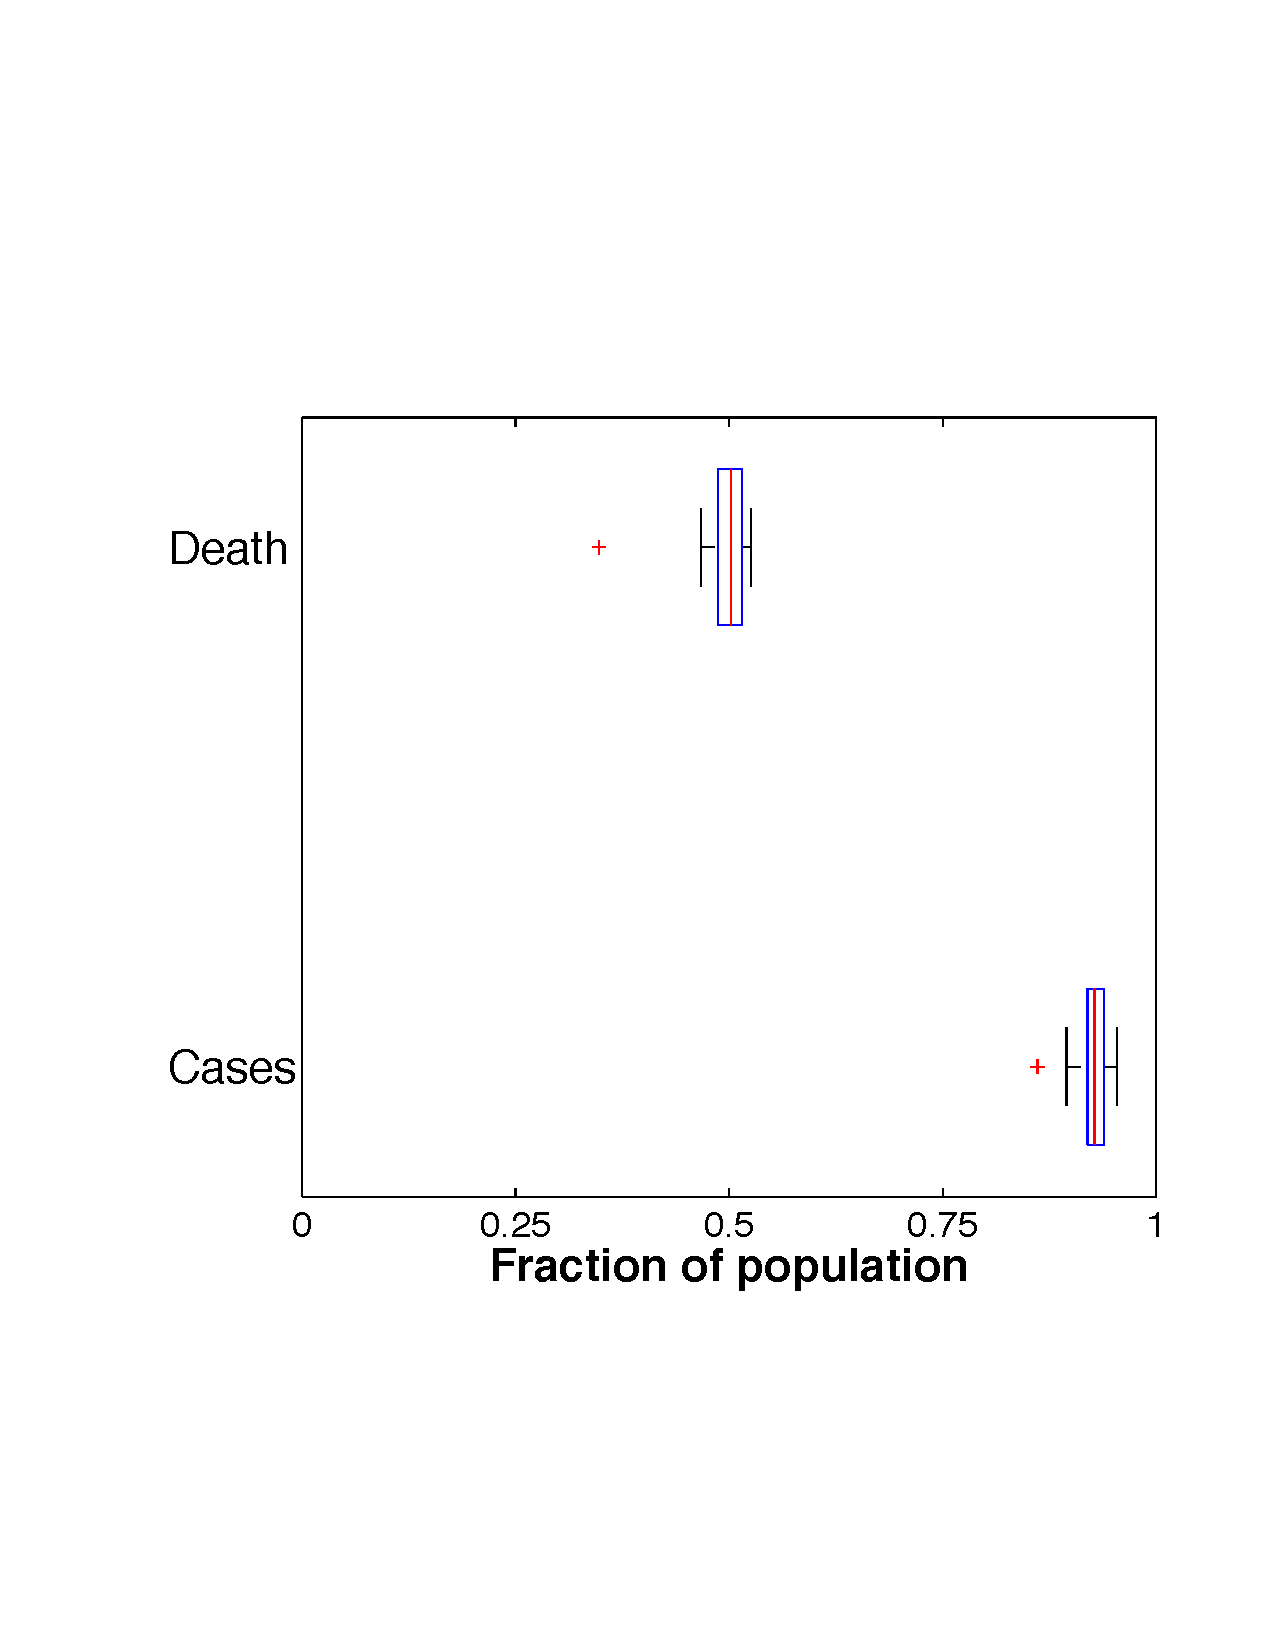
\includegraphics[width = 0.5\textwidth]{BWplot.pdf}

\end{figure}
\end{frame}

\begin{frame}
\frametitle{Trajectories of S, D and R}
\begin{figure}
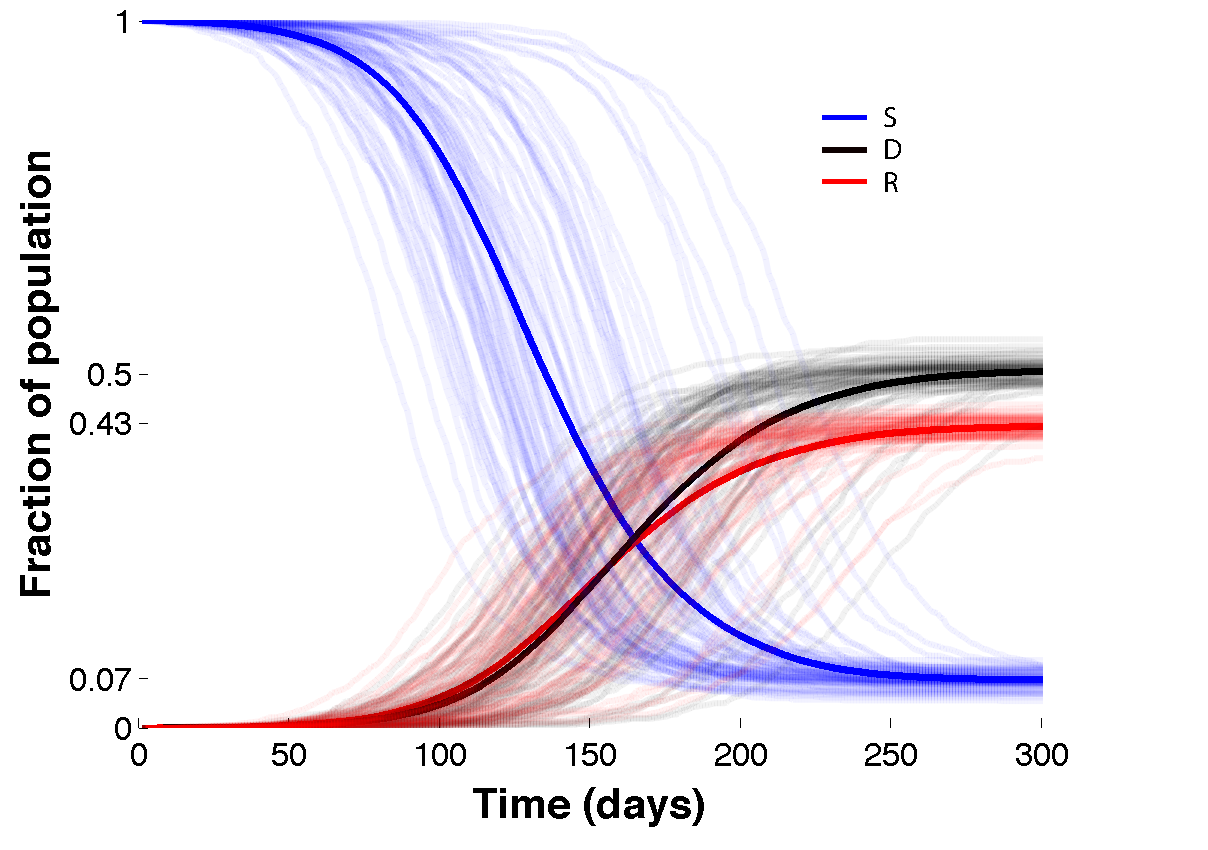
\includegraphics[width = 0.7\textwidth]{SDRcurves.pdf}
\end{figure}
\end{frame}



\begin{frame}
\frametitle{Results of Intervention}
\hspace{-.4cm}
\begin{adjustbox}{max totalsize={1.1\textwidth}{\textheight},center}
\def\angle{0}
\def\radius{3}
\def\cyclelist{{"blue","red","green","green"}}
\newcount\cyclecount \cyclecount=-1
\newcount\ind \ind=-1
\begin{tikzpicture}[scale=.8]
\draw[white] (-1,-4) rectangle (3.5,3.5);
\node at (0,3.5) {\Large With Intervention};
  \foreach \percent/\name in {
      96/S (96\%),
      2/D (2\%),
      2/R (2\%)
    } {
      \ifx\percent\empty\else               % If \percent is empty, do nothing
        \global\advance\cyclecount by 1     % Advance cyclecount
        \global\advance\ind by 1            % Advance list index
        \ifnum3<\cyclecount                 % If cyclecount is larger than list
          \global\cyclecount=0              %   reset cyclecount and
          \global\ind=0                     %   reset list index
        \fi
        \pgfmathparse{\cyclelist[\the\ind]} % Get color from cycle list
        \edef\color{\pgfmathresult}         %   and store as \color
        % Draw angle and set labels
        \draw[fill={\color!50},draw={\color}] (0,0) -- (\angle:\radius)
          arc (\angle:\angle+\percent*3.6:\radius) -- cycle;
        %\node at (\angle+0.5*\percent*3.6:0.85*\radius) {\percent\,\%};
        \node[pin=\angle+0.5*\percent*3.6:\name]
          at (\angle+0.5*\percent*3.6:\radius) {};
        \pgfmathparse{\angle+\percent*3.6}  % Advance angle
        \xdef\angle{\pgfmathresult}         %   and store in \angle
      \fi
    };
\end{tikzpicture}
\begin{tikzpicture}[scale=.8]
\draw[white] (-3,-4) rectangle (3.5,3.5);
	\node at (0,3.5) {\Large Without Intervention};
  \foreach \percent/\name in {
      7/S (7\%),
      50/D (50\%),
      43/R (43\%)
    } {
      \ifx\percent\empty\else               % If \percent is empty, do nothing
        \global\advance\cyclecount by 1     % Advance cyclecount
        \global\advance\ind by 1            % Advance list index
        \ifnum3<\cyclecount                 % If cyclecount is larger than list
          \global\cyclecount=0              %   reset cyclecount and
          \global\ind=0                     %   reset list index
        \fi
        \pgfmathparse{\cyclelist[\the\ind]} % Get color from cycle list
        \edef\color{\pgfmathresult}         %   and store as \color
        % Draw angle and set labels
        \draw[fill={\color!50},draw={\color}] (0,0) -- (\angle:\radius)
          arc (\angle:\angle+\percent*3.6:\radius) -- cycle;
        %\node at (\angle+0.5*\percent*3.6:0.85*\radius) {\percent\,\%};
        \node[pin=\angle+65+0.5*\percent*3.6:\name]
          at (\angle+0.5*\percent*3.6:\radius) {};
        \pgfmathparse{\angle+\percent*3.6}  % Advance angle
        \xdef\angle{\pgfmathresult}         %   and store in \angle
      \fi
    };
\end{tikzpicture}
\end{adjustbox}
\end{frame}



%\begin{frame}
%\frametitle{Spatial Agent Model}
%\section{Spatial}
%\begin{itemize}
%\item Why we should incorporate the spatial info?
%\begin{itemize}
%\item We have different contact ratios within households, communities and funerals ($\beta_H$, $\beta_C$, $\beta_F$)
%\item Travel patterns are distinct among big cities and small villages
%\end{itemize}
%\item show the Flow Chart Models
%\item go into the details of the model
%\begin{itemize}
%\item How people get infected (3 different scenarios: househoulds, communities and funerals)
%\item How people travel (every one has prob 0.2 to travel, those away from home will return w/ prob 0.5, while the others have higher chance to travel locally, different probabilities based on the density of the cities/villages for non-local travellers)
%\end{itemize}
%\item Figures $\&$ results
%\end{itemize}
%
%\end{frame}

%\begin{frame}{Spatial Importance}
%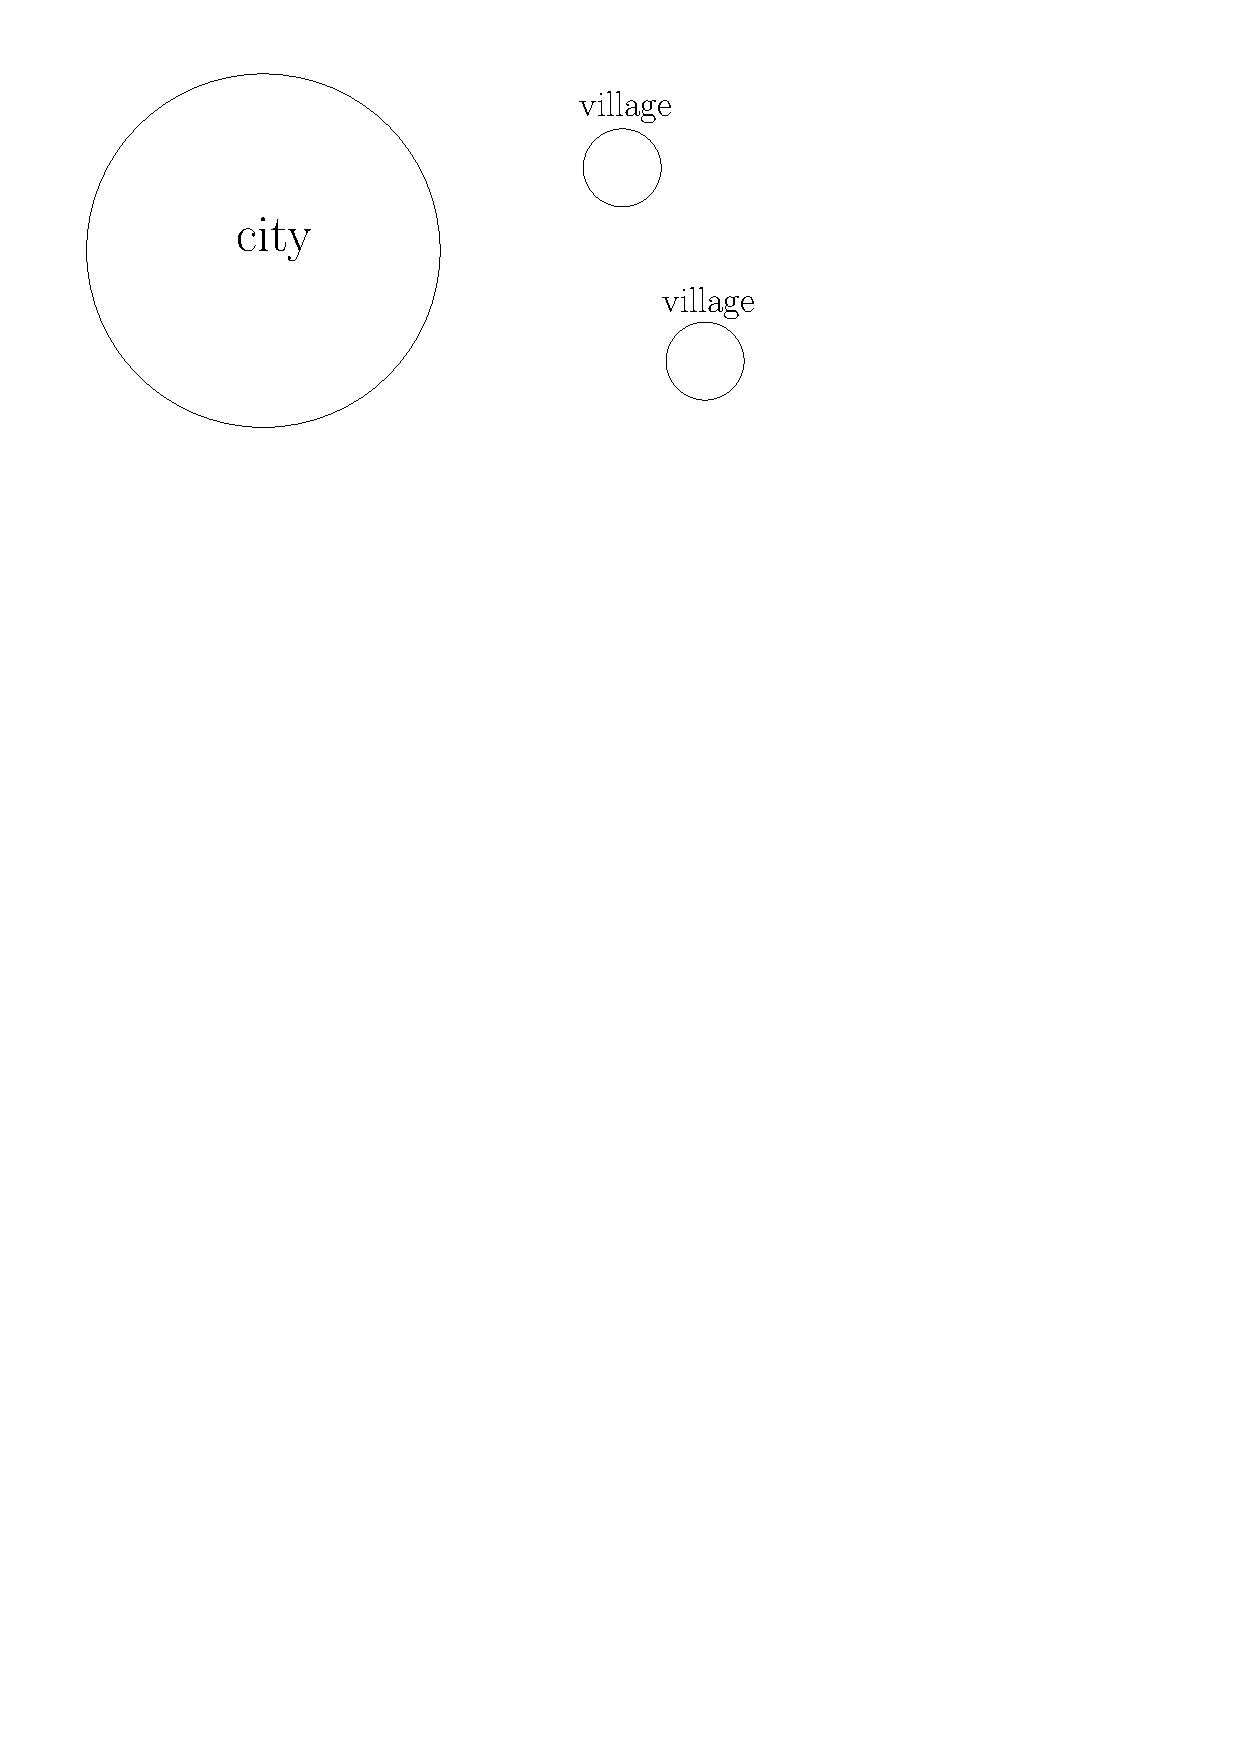
\includegraphics[width=\textwidth]{cities}
%\end{frame}
%\draw[fill=black] (1,1) rectangle (2,2);

%\begin{frame}{States and Transitions}
%\begin{figure}[h!]
%\begin{center}
%\begin{tikzpicture}[->,shorten >=1pt,auto,node distance=3cm,
%  thick,main node/.style={circle,fill=blue!20,draw,font=\sffamily\Large\bfseries}]
%
%  \node[main node] (1) {S};
%  \node[main node] (2) [right of=1] {E};
%  \node[main node] (3) [right of=2] {I};
%  \node[main node] (4) [right of=3] {F};
%  \node[main node] (5) [below of=3] {H};
%  \node[main node] (6) [below of=4] {D};
%  \node[main node] (7) [left of=5] {R};
%
%  \path[every node/.style={font=\sffamily\small}]
%    (1)
%        edge node {} (2)
%        %edge [loop above] node {$1-p_{SE}$} (1)
%    (2) 
%        edge node {} (3)
%        % edge [loop above] node {} (2)
%      
%    (3) 
%       edge node {} (4)
%       edge node[right] {} (5)
%       edge node[left] {} (7)
%        %edge [loop above] node {$p_{II}$} (3)
%    (4)
%         edge node {} (6)
%        % edge [loop above] node {$p_{FD}$} (6)
%       
%(5) edge node{} (6) 
%	edge node {} (7)
%%edge [loop below] node {$p_{FF}$} (6)     
%;
%        
%\end{tikzpicture}
%\end{center}
%\caption{States and transitions for individuals.}
%\label{fig:sabm-states}
%\end{figure}
%\end{frame}

\begin{frame}{Spatial Agent-Based Model: Overview}
\begin{itemize}
\item City residents normally distributed
\item Family, community, and funeral spread rates
\item Family goes home for funeral
\item Neighbors at their home can attend funeral
\item Hospital is quarantined
\item Probability and transition time between states
\end{itemize}
\end{frame}

\begin{frame}{Regions of Infection Spread}
%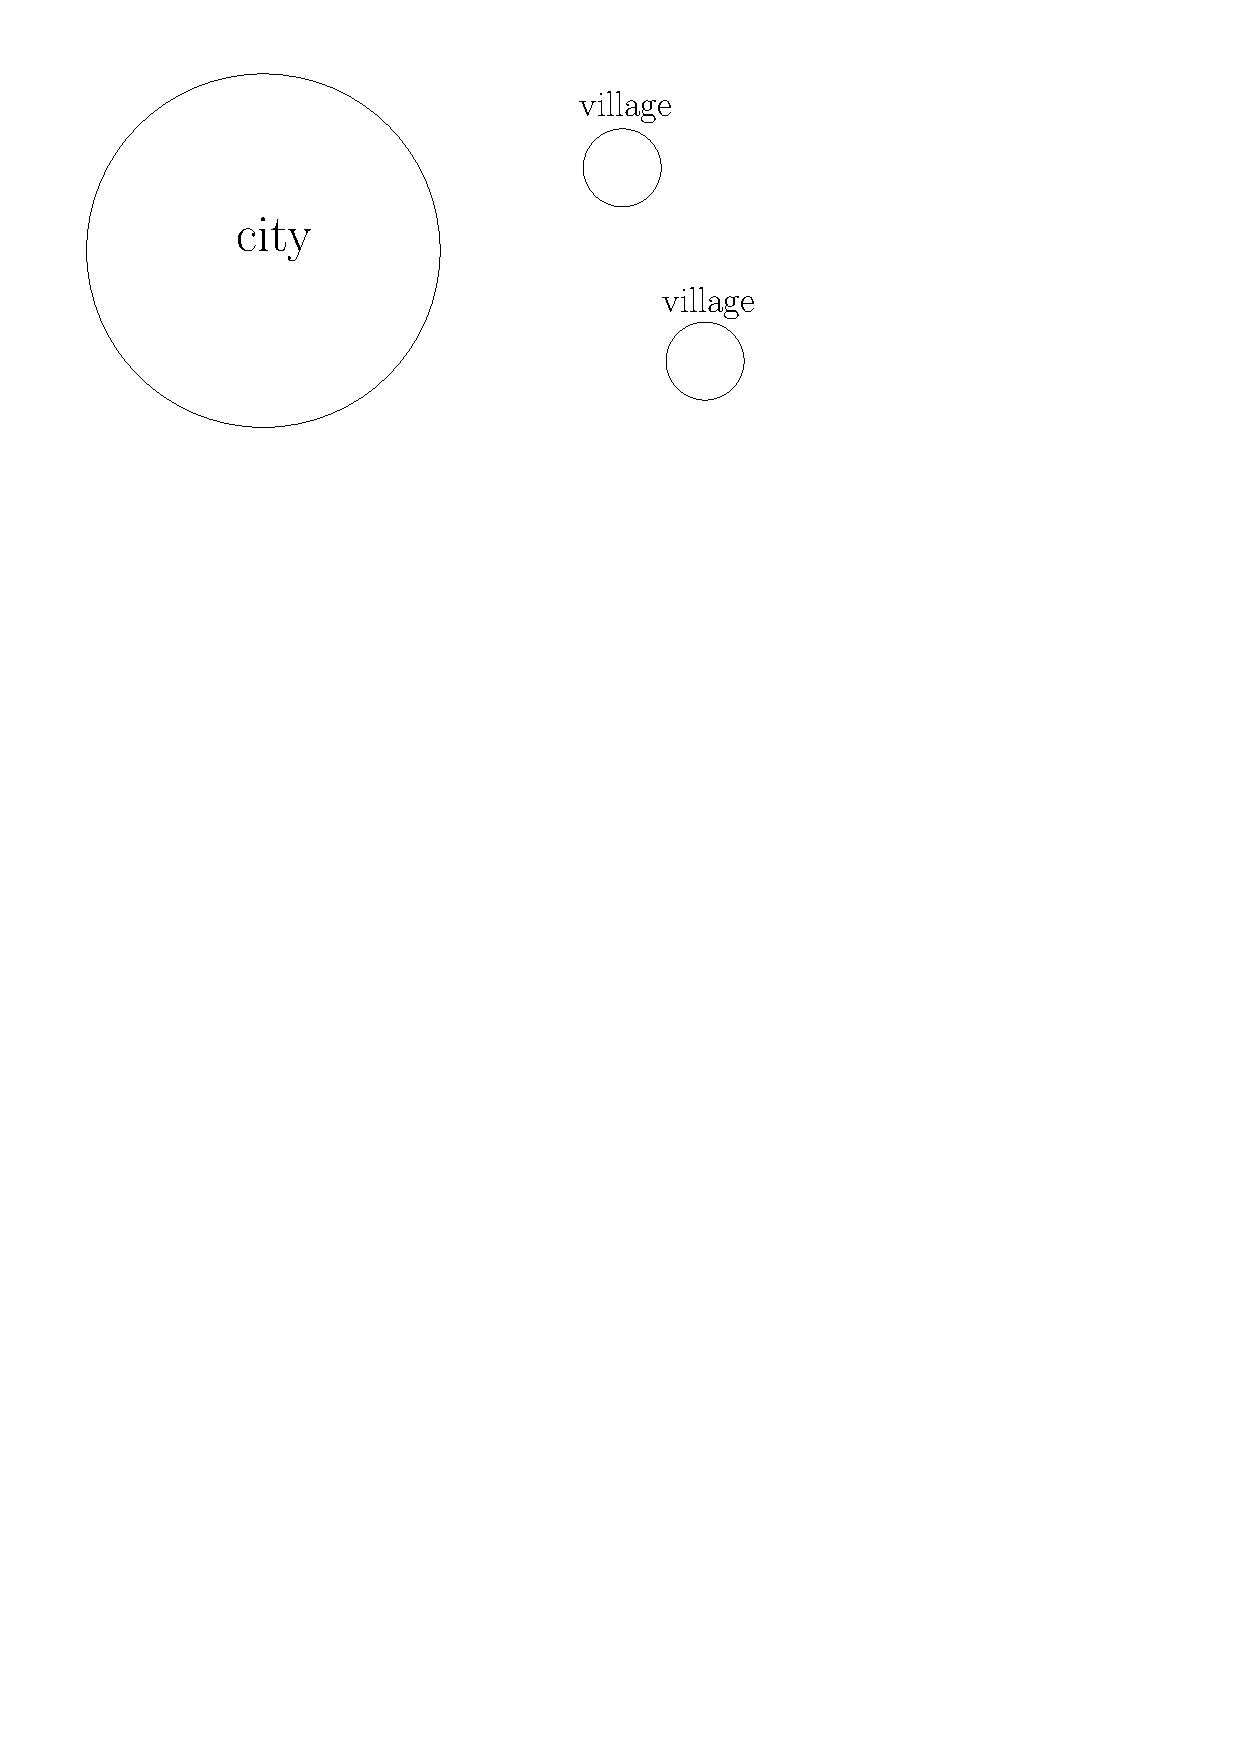
\includegraphics[width=\textwidth]{cities}
\begin{figure}[h!]
\begin{center}
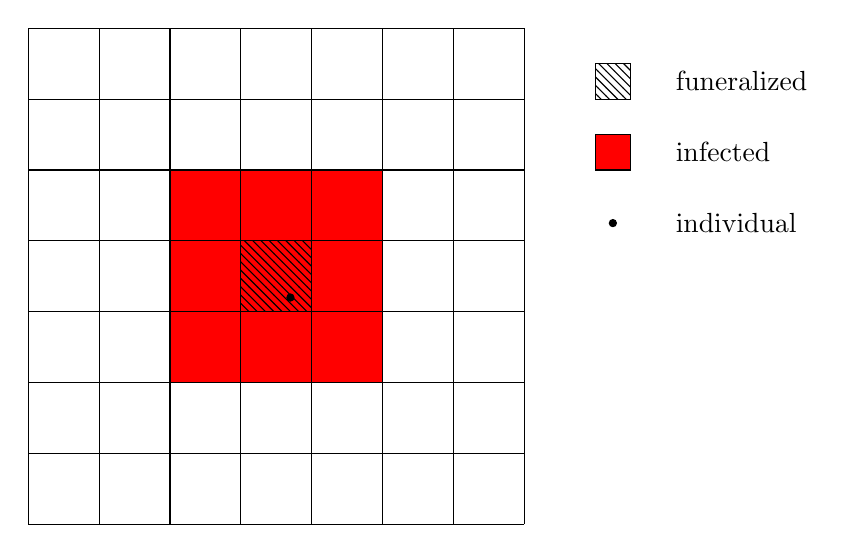
\begin{tikzpicture}[scale=.9]
\draw [fill=red] (0,0) rectangle (3,3);
\draw[pattern=north west lines, pattern color=black] (1,1) rectangle (2,2);
\draw[step=1cm, thin] (-2,-2) grid (5,5);
\draw[fill=black] (1.7,1.2) circle (.05cm);

\draw[pattern=north west lines, pattern color=black] (6,4) rectangle (6.5,4.5);
\node[anchor=west] at (7,4.25) {funeralized};
\draw[fill=red] (6,3) rectangle (6.5,3.5);
\node[anchor=west] at (7,3.25) {infected};
\draw[fill=black] (6.25,2.25) circle (.05cm);
\node[anchor=west] at (7,2.25) {individual};
\end{tikzpicture}
\end{center}
\label{fig:sabm-states}
\end{figure}
\end{frame}

\begin{frame}{Available Travel Routes}
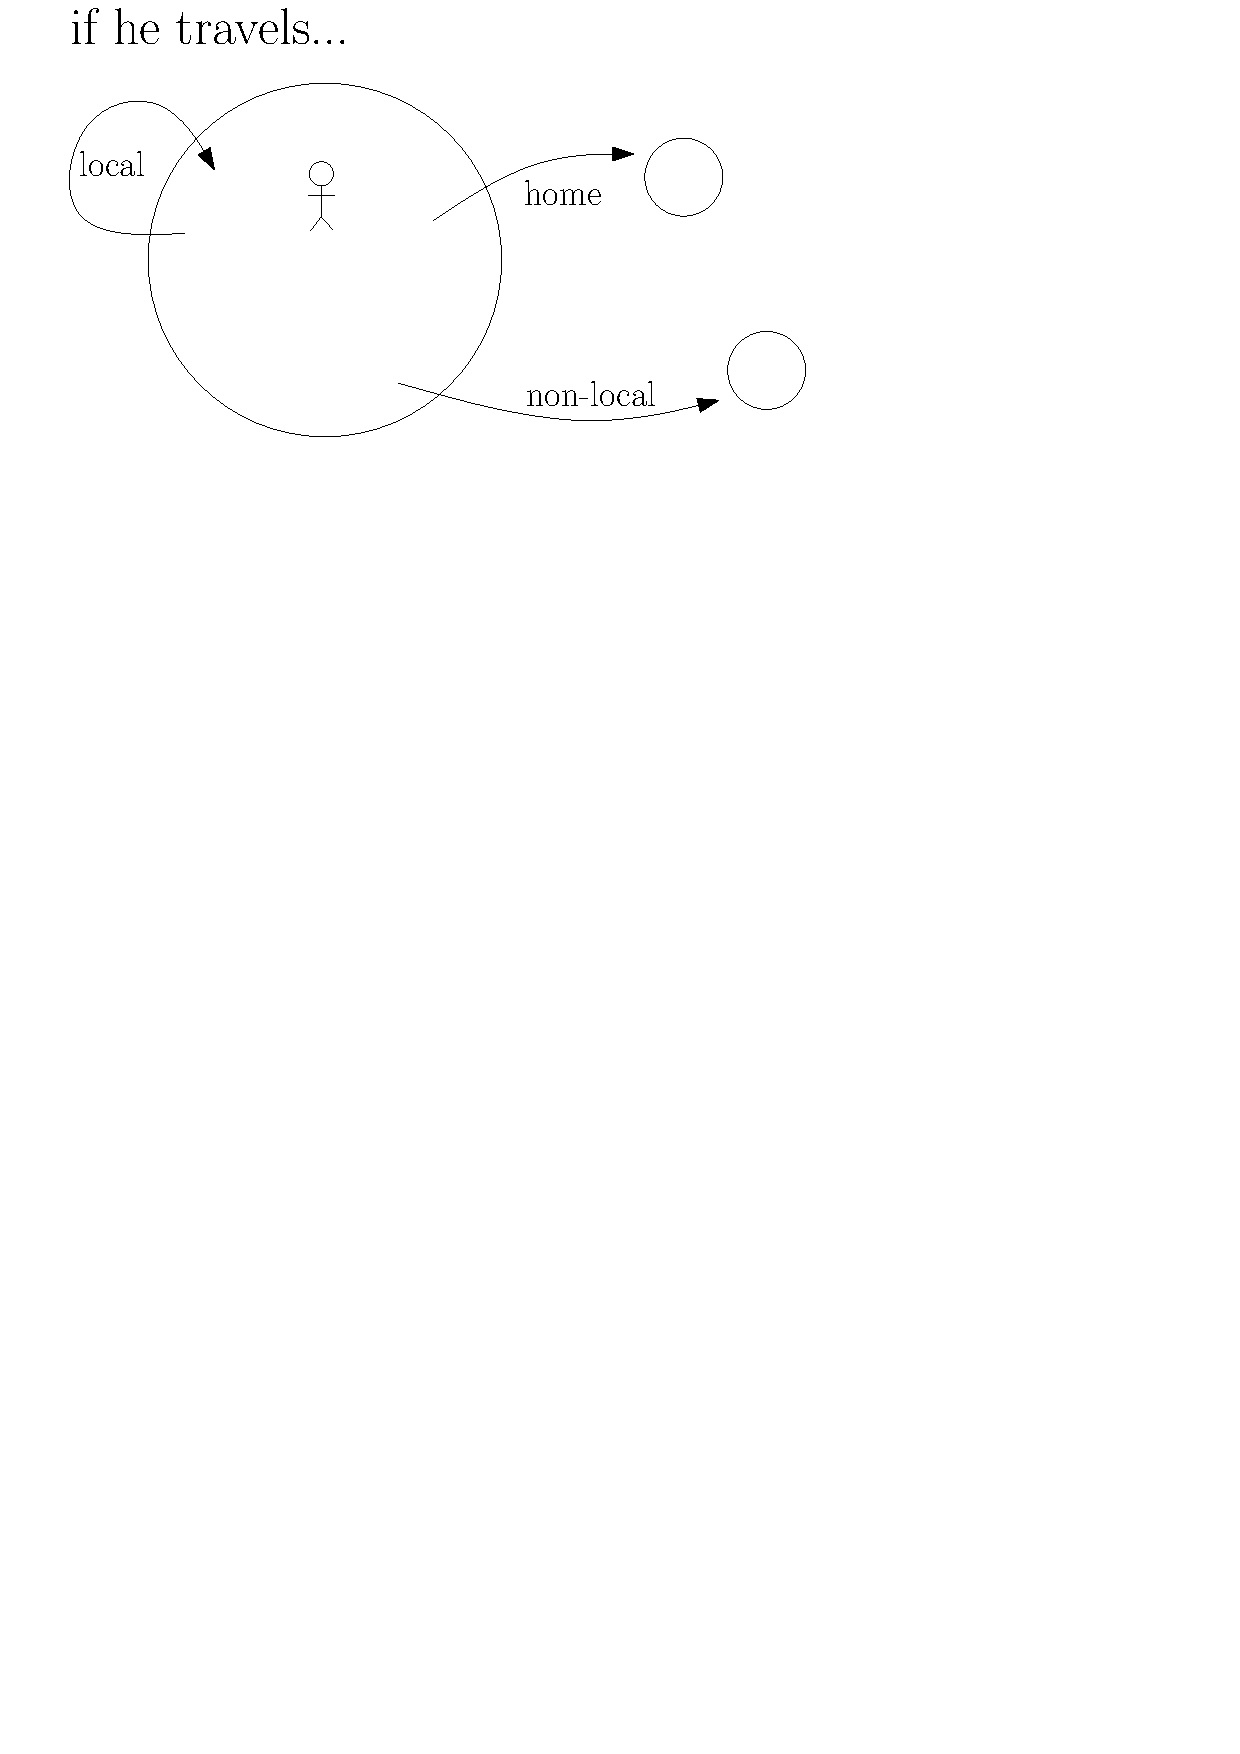
\includegraphics[width=\textwidth]{travel}
\end{frame}


\begin{frame}
\frametitle{Trajectories of S, R, D: 100 simulations}
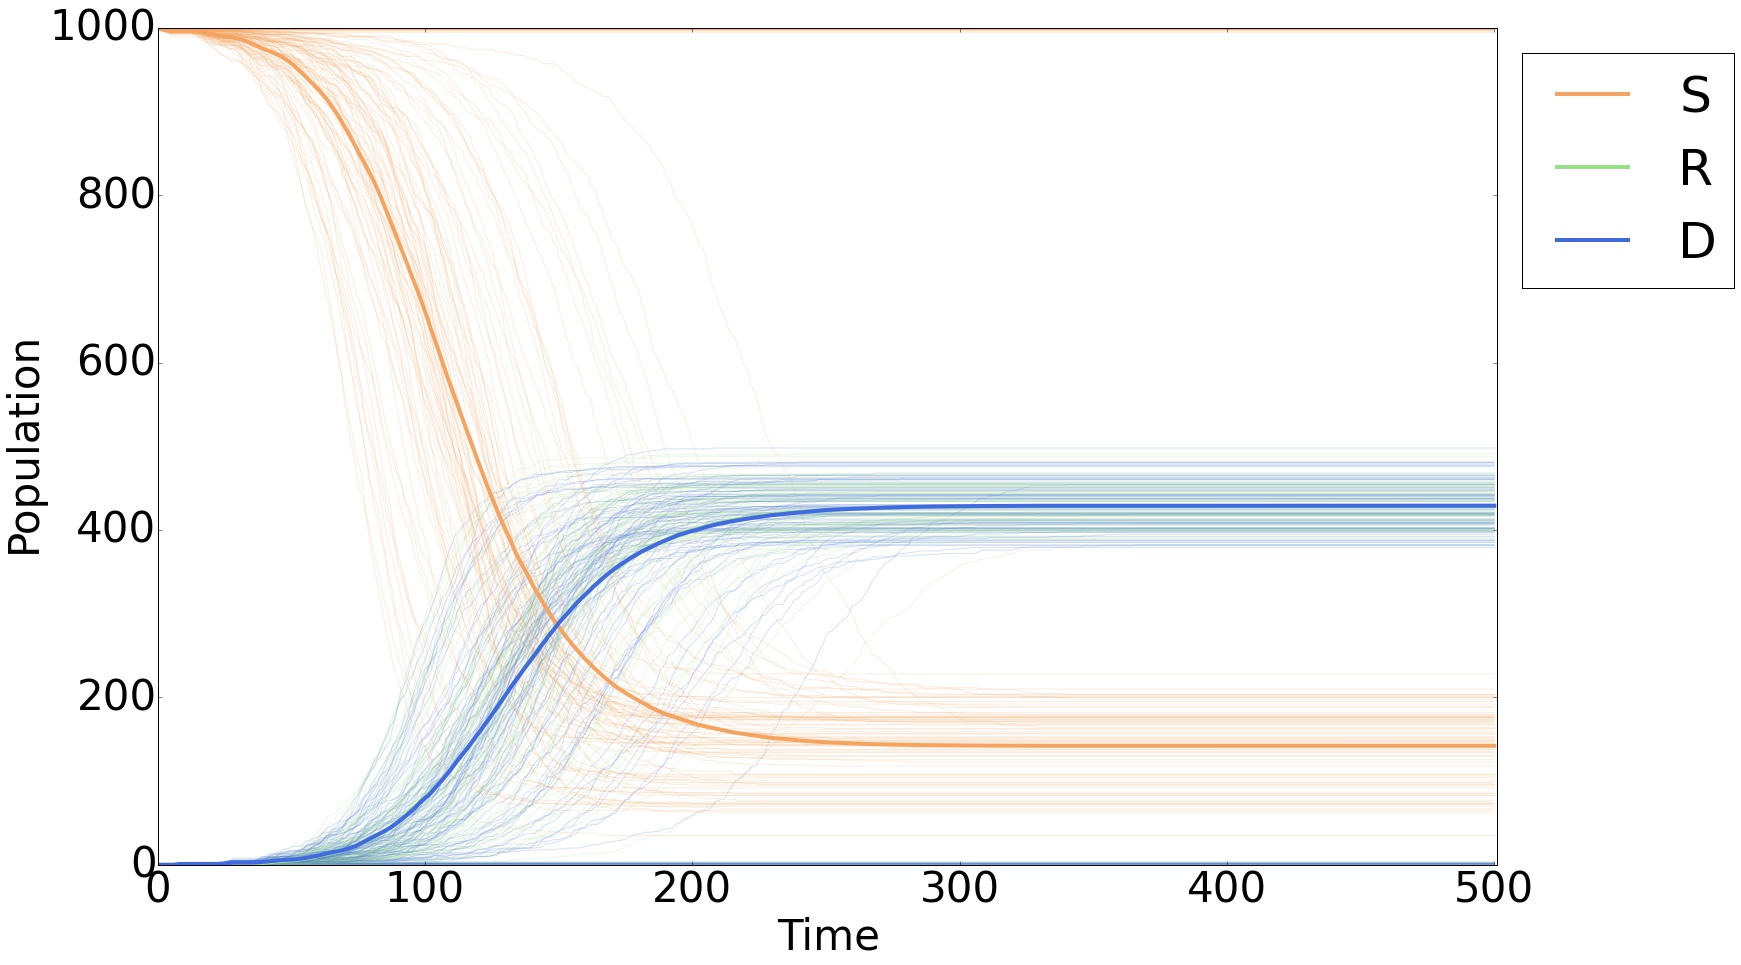
\includegraphics[width=\textwidth]{average-time-series}
\end{frame}

\begin{frame}
\frametitle{Probability of an Outbreak}
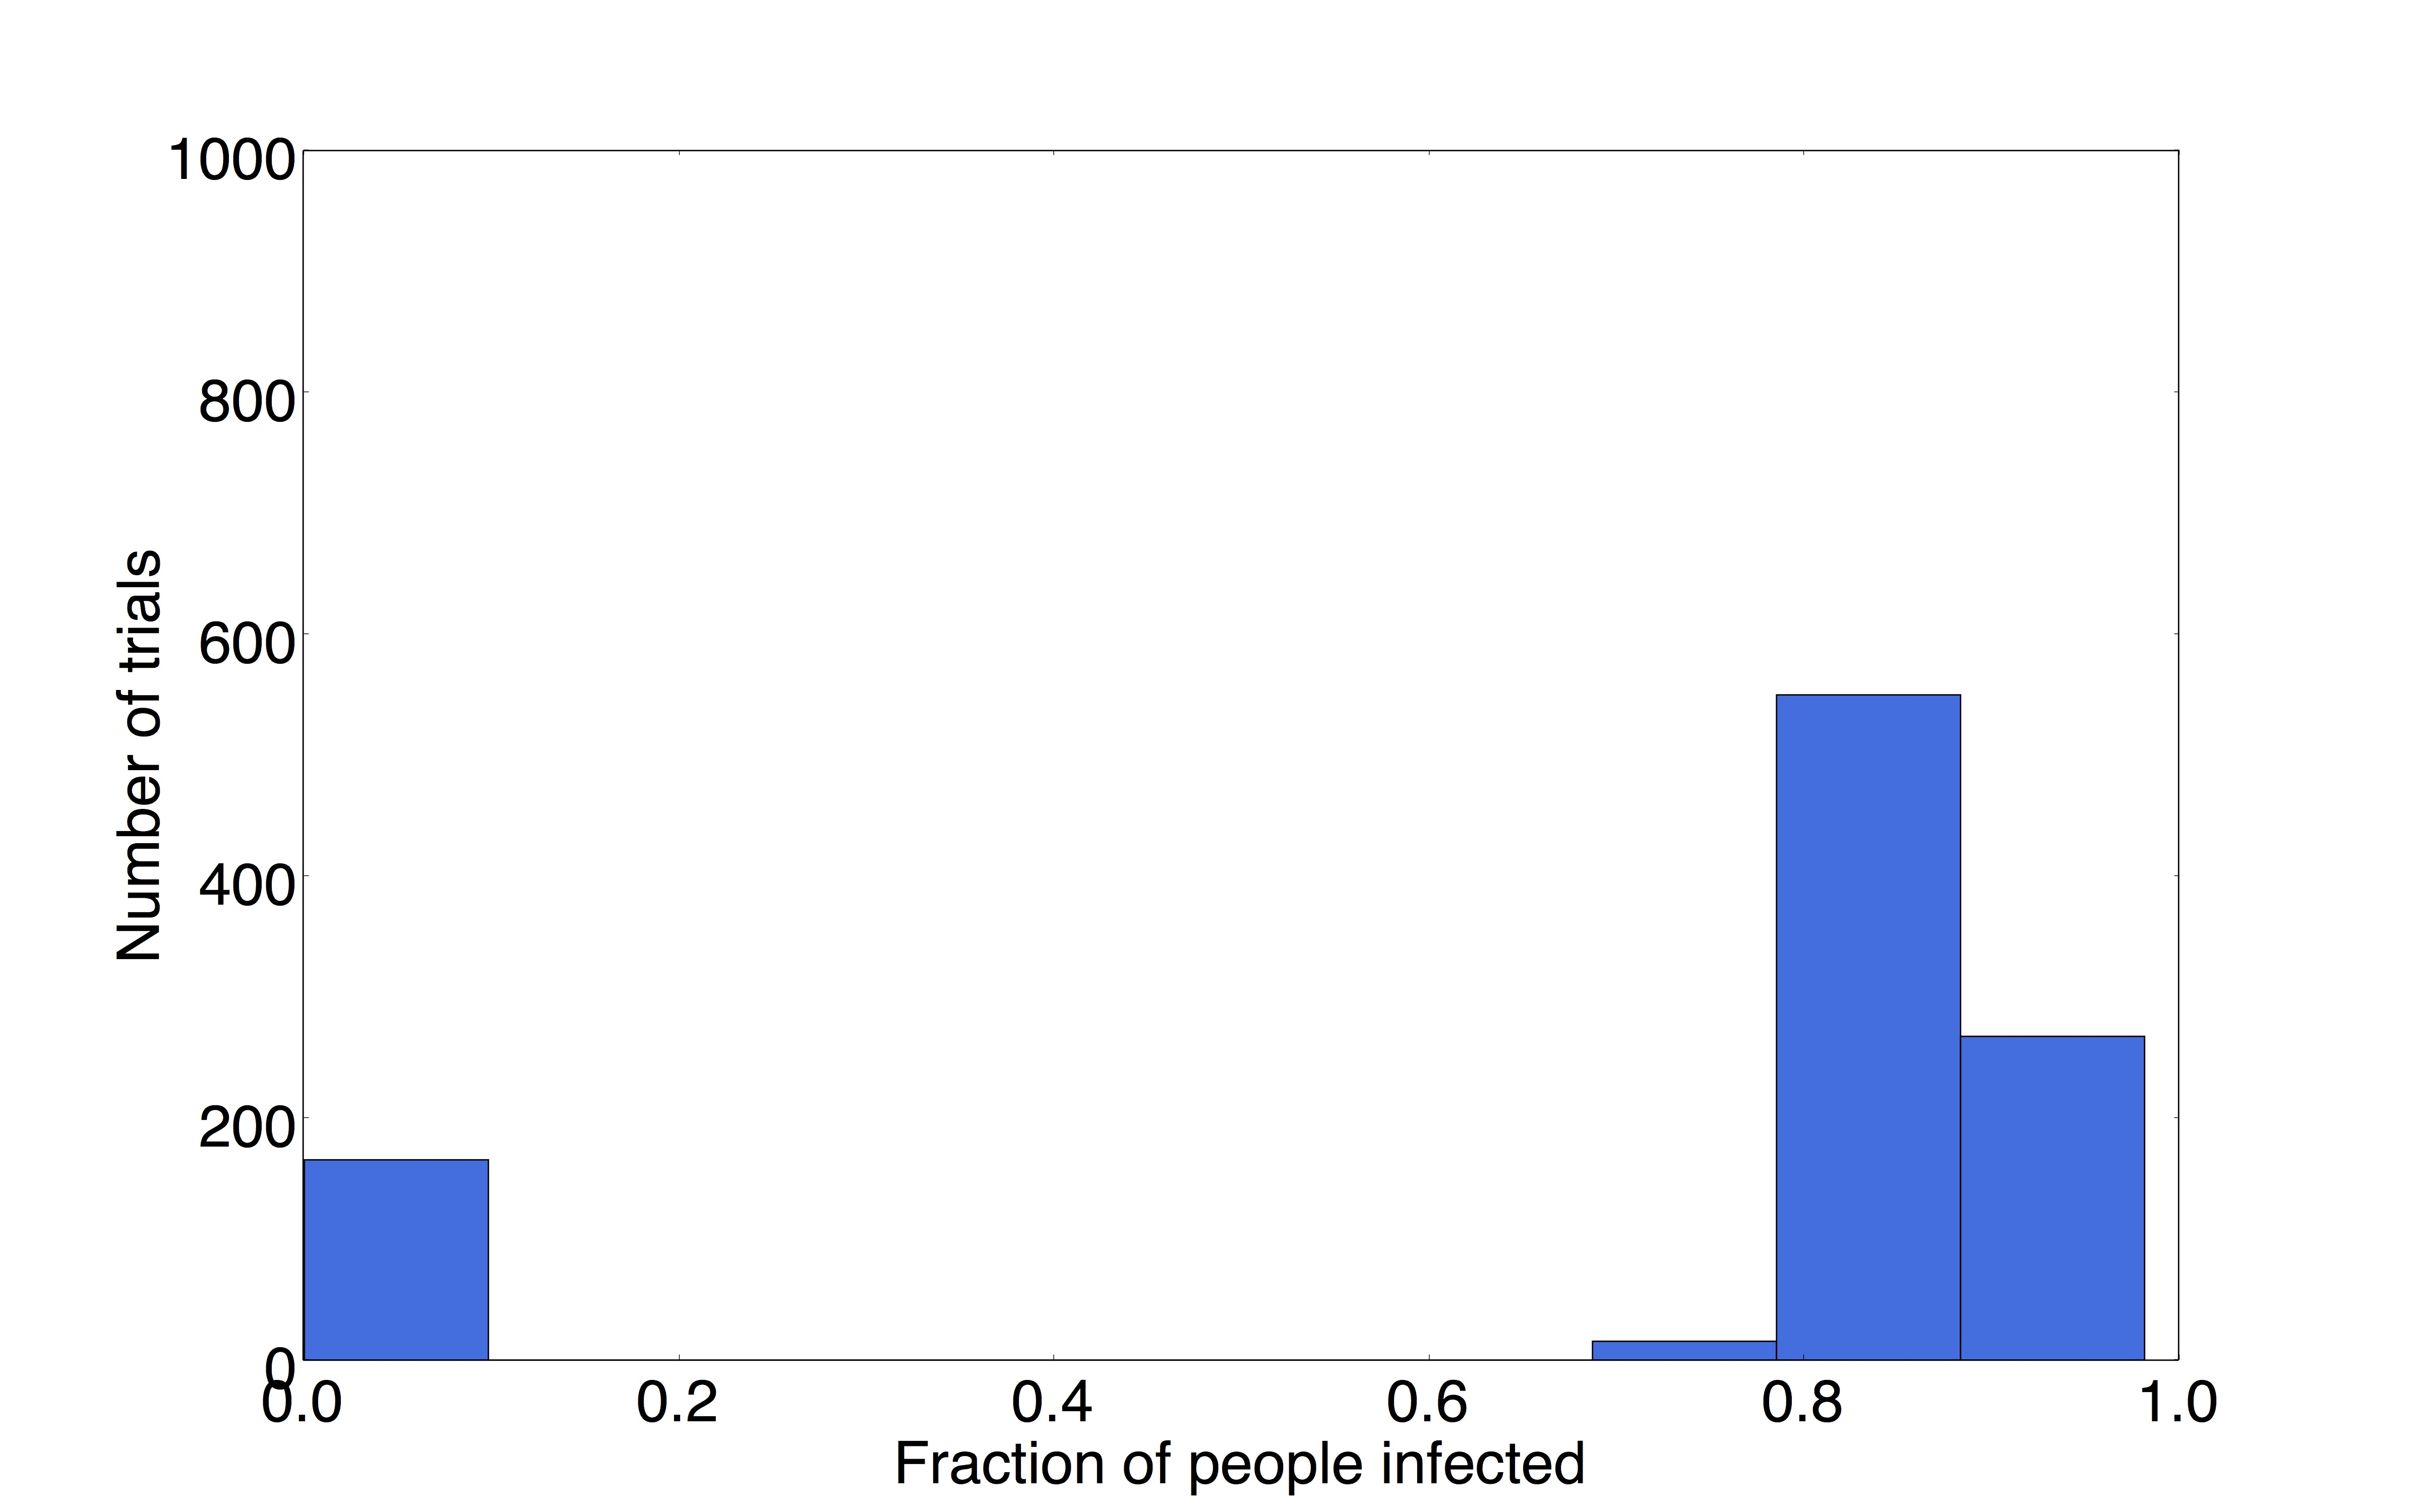
\includegraphics[width=\textwidth]{Histogram-sabd}
\end{frame}


\begin{frame}
\frametitle{Summary}
\section{Summary}
\begin{itemize}
\item Deterministic and probabilistic approaches give similar results
\item Incorporating spatial information is useful
\item Intervention has a big effect:
\begin{itemize}
\item Over 90 percent contract the disease
\item About 50 percent dies due to disease
\item Intervention causes these figures to decrease significantly 
\end{itemize}
\end{itemize}
\end{frame}


\end{document}
